\documentclass[10pt]{article}
\usepackage[english]{babel}
\usepackage[parfill]{parskip}
\usepackage{float}
\usepackage{hyperref}
\usepackage{multirow}
\usepackage{xcolor}
\usepackage{todonotes}
\usepackage{amsmath}
\usepackage[margin=1.3in]{geometry}
\usepackage{array}
\usepackage{graphicx}
\usepackage{caption, subcaption}
\usepackage{enumitem}
\usepackage{tabularx}
\usepackage{lmodern}
% \usepackage[fontsize=9pt]{scrextend}
\usepackage[noend]{algorithm2e}


\setlength{\parskip}{1em}

\makeatletter
\renewcommand{\rmdefault}{\sfdefault}
% \def\subtitle#1{\gdef\@subtitle{#1}}

\def\leftHeader#1{\listadd\@leftHeader{#1}}
\def\rightHeader#1{\listadd\@rightHeader{#1}}

\def\@maketitle{
    \renewcommand{\do}[1]{##1

    }
    \begin{minipage}[t]{5cm}
        \flushleft
        \dolistloop{\@leftHeader}
    \end{minipage}
    \hfill
    \begin{minipage}[t]{5cm}
        \flushright
        \dolistloop{\@rightHeader}
    \end{minipage}
    \centering

    \vspace{0.7cm}
% \vfill
    {\huge\bfseries\@title\par}
% \vfill
    \vspace{0.7cm}
    \thispagestyle{empty}
}
\makeatother

\newcommand{\one}[1]{\colorbox{yellow}{$\displaystyle #1$}}
\newcommand{\two}[1]{\colorbox{green}{$\displaystyle #1$}}

\newcommand{\onen}[1]{\colorbox{yellow}{#1}}
\newcommand{\twon}[1]{\colorbox{green}{#1}}

\title{Fundamental project\\\LARGE Gradient-Free Policy Optimisation}
\leftHeader{Ward Gauderis}
\leftHeader{0588485}
\rightHeader{Reinforcement Learning}
\rightHeader{Faculteit Wetenschappen}
\rightHeader{Vrije Universiteit Brussel}
\leftHeader{01/06/2023}

\begin{document}
\maketitle

\section{Introduction}
The goal of reinforcement learning is to learn a policy that maximises the expected cumulative
reward of an agent in a given environment.\\
There exist multiple approaches to this problem, but in this project
we focus on searching directly for an optimal parametric policy in the policy space
spanned by the parameters of the policy.
This is a challenging problem, as the policy space is often very large and has many local optima,
but stochastic (local) search methods have been shown to be very effective in finding relatively good policies in a reasonable amount of time.
If the policy space is continuous and differentiable, gradient-based methods like gradient-descent can be used to find the optimal policy.
But also gradient-free methods, more commonly used in the context of heuristic combinatorial
optimisation, are still applicable in the context of reinforcement learning.\\
In this project we implement two gradient-free optimisation algorithms, zeroth-order optimisation and population-based optimisation, investigate the influence of their hyper-parameters and compare their performance.\\
We do this by applying the algorithms to the 'Lunar Lander' task from the OpenAI Gym \cite{gym} in which
the agents goal is to land a simple spaceship smoothly on a flat surface by controlling the main engine and the two side thrusters.

In the following sections we first introduce policy-free reinforcement learning, then we discuss the two algorithms we implement and our experimental setup before we present our experimental results and
discuss them.

\section{Literature Review}

Many fundamental reinfocement learning algorithms like Q-learning or SARSA rely exclusively on value function
estimation to learn a solution to the Bellman equation and directly derive a policy from this learned value function. This class of algorithms is called critic-only since they use the value function as a critic to evaluate the quality of the possible action in a given state.\\
An alternative solution is to work with parametrised policies and search directly in the policy space
for an optimal solution. These algorithms use stochastic (local) search on the parameters of the
actor's policy and are therefore called actor-only algorithms.\\
In state-of-the-art reinfocement learning, often these two approaches are combined in so called actor-critic algorithms in order to combine the advantages of both.
\cite{slides}

In this project we focus on actor-only algorithms.
They have the advantage over critic-only methods in that they can be applied straightforwardly to continuous action spaces and have the potential to learn more efficiently in the case when the value function is not easily approximated.
Because of the explicit policy representation, actor-only algorithms can also be provided with prior knowledge about a task and can even learn stochastic policies.
This comes with the addditional benefit that they can learn appropriate levels
of exploration automatically and approach deterministic policies asymptotically.
\cite{RL}

When the policy representation is continuous and differentiable, gradient-based stochastic search methods
can be used to find the optimal policy.
A stochastic estimate whose expectation approximates the gradient
of the (unknown) reward function with respect to the policy parameters can then be used to update the policy using
gradient ascent with the objective of maximising the expected cumulative reward per episode.
The methods that use this approach are called policy-gradient methods.\\
Within this class of methods, we can further distinguish between deterministic and stochastic policy-gradient methods.
Stochastic methods predict probability distributions over the action space and sample from these distributions to determine the next action, while deterministic methods directly predict the next action.
But both method always require some way to estimate the gradient of the reward function, in which lies the main challenge.\\
Policy gradient methods essentially only use local information contained in the estimated gradient to update the policy. This brings multiple problems with it, even though it can achieve high-quality solutions.
Policy gradient methods are sample inefficient, as they require a large number of samples to estimate the gradient and even then the gradient estimate is often noisy with a high variance. And because they only use local information based on the previous gradient estimate, they can get stuck in local optima
and are not able to reuse information from previous iterations.
\cite{slides, RL}

A large class of stochastic search methods completely avoids relying on gradient information.
These gradient-free methods are often used to solve combinatorial optimisation problems heuristically, but can also be applied to reinforcement learning.
In theory and in the limit of running time, gradient-free methods often can achieve globally optimal solutions, but in practice they are more successful in finding high-quality solutions in a reasonable amount of time.\\
Stochastic local search methods that do not depend on gradient calculation instead rely on perturbations
of existing sub-optimal policies to iteratively improve them. Every time a perturbed policy is
created, it is evaluated in the environment and based on the reward obtained, the parameters of the policy are updated.
Some important examples of gradient-free methods are:
\begin{itemize}
    \item \textbf{Simulated annealing}: a hill-climbing method that uses a decreasing temperature
          parameter to control the size of the perturbations.
    \item \textbf{Particle swarm optimisation}: a population-based method that uses a population of
          policies to iteratively improve them.
    \item \textbf{Evolutionary algorithms}: population-based methods inspired by biological evolution that apply genetic operators such as mutation, recombination and selection between multiple policies.
\end{itemize}
These methods might be able to escape some local optima that gradient-based methods get stuck in, but are still not guaranteed to find the global optimum. Next to that, they are also not more sample efficient as every perturbation still needs to be evaluated. However, they are often much easier to 
design and implement and can be fine-tuned to task at hand to achieve high-quality solutions very fast.
\cite{HO}

\section{Methods}

To solve 'Lunar Lander' task,
we employ two gradient-free optimisation algorithms:
zeroth-order optimisation and population-based optimisation.
Both methods build on the idea of iteratively perturbing the parameters of the policy and evaluating the resulting policies
in an attempt to find the parameters maximising the expected cumulative reward of the task.
Important hyper-parameters of both algorithms are the size $\sigma$ of the perturbations, which can influence the convergence
speed of the algorithm as well as the quality of the resulting policy, and the number $E$ of evaluation episodes, which determines
how much randomness is introduced in the evaluation of the policies.
Both parameters can be tuned to balance exploration and exploitation in the algorithms.

In my implementation of zeroth-order optimisation \ref{alg:zeroth}, at every iteration of the algorithm the parameters of the policy
are perturbed by a random vector sampled from a multivariate normal distribution with mean $\mathbf{0}$ and covariance matrix $\sigma^2 I$
so that all individual perturbations are identically distributed and independent.
The perturbation is then applied in both the positive and negative direction and the resulting policies are evaluated.
The final policy of every iteration is then obtained by adding a linear interpolation
of the positive and negative perturbations to the parameters of the initial policy, depending on their evaluation returns.
This update is multiplied by the learning rate $\alpha$ to control how much the parameters are updated at every iteration,
similar to the influence of $\sigma$.

\begin{algorithm}[h]
    \KwIn{$\pi_\theta$: parametric policy}
    \KwIn{$\sigma$: standard deviation}
    \KwIn{$E$: number of evaluation episodes}
    \KwIn{$\alpha$: learning rate}
    \SetKwBlock{Loop}{Loop}{EndLoop}
    \Loop{
        sample $p \sim \mathcal{N}(\mathbf{0}, \sigma^2 I)$

        $r^+ \gets \text{evaluate}(\pi_{\theta+p}, E)$

        $r^- \gets \text{evaluate}(\pi_{\theta-p}, E)$

        $\Delta \gets \frac{r^+ - r^-}{2} p$

        $\pi_\theta \gets \pi_{\theta+\alpha\Delta}$}

    \caption{Zeroth-order optimisation}
    \label{alg:zeroth}
\end{algorithm}

The population-based optimisation algorithm \ref{alg:population} no longer depends on a learning rate $\alpha$ but instead uses
a population of $N$ policies. At every iteration, $N$ policies are created by perturbing the parameters of the initial policy
with a random vector sampled from the same distribution as in zeroth-order optimisation.
Each one is evaluated separately and the policy with the highest evaluation return is selected as the final policy of the iteration.

\begin{algorithm}[h]
    \KwIn{$\pi_\theta$: parametric policy}
    \KwIn{$\sigma$: standard deviation}
    \KwIn{$E$: number of evaluation episodes}
    \KwIn{$N$: population size}
    \SetKwBlock{Loop}{Loop}{EndLoop}
    \SetKwFor{RepTimes}{repeat}{times}{end}
    \Loop{
        $r_\text{max} \gets -\infty$

        \RepTimes{$N$}{
            sample $p \sim \mathcal{N}(\mathbf{0}, \sigma^2 I)$

            $r \gets \text{evaluate}(\pi_{\theta+p, E})$

            \If{$r \ge r_\text{max}$}{
                $r \gets r_\text{max}$

                $\pi_\theta \gets \pi_{\theta+p}$
            }
        }
    }
    \caption{Population-based optimisation}
    \label{alg:population}
\end{algorithm}

Both algorithms were run for 10\,000 iterations in the gym environment 'Lunar Lander' with a time limit of 500 steps per episode.
This limit was chosen to encourage the agents to learn efficient policies and avoid long simulation times while providing enough
to solve every episode. An episode is considered to be solved by an agent when a cumulative reward above 200 is obtained.\\
A continuous version of the gym environment was used, which means that the agent can control the thrust of the main engine and the lateral boosters. While the observation space is described by 8 continuous values, the action space is defined by 2 continuous values between -1 and 1.\cite{gym}\\
For this reason, we design our parametric policy to be a multilayer perceptron with one hidden layer of
128 neurons while the output layer has two neurons with a hyperbolic tangent activation function.
The policy network is implemented in PyTorch.\cite{pytorch}

After reasonable fine-tuning of the hyper-parameters, the following values were found to be suitable for the zeroth-order method:
\begin{itemize}
    \item Standard deviation of the perturbation $\sigma=0.05$
    \item Number of evaluation episodes $E = 1$
\end{itemize}
In the experimental results, we investigate the influence of the number of evaluation episodes $E$ on the performance of the agent.

For the population-based method, the size of the perturbations was decreased and we will research the combined impact of the population size
$N$ and number of evaluation episodes $E$ on the results:
\begin{itemize}
    \item Standard deviation of the perturbation $\sigma=0.01$
\end{itemize}

\section{Results}

In this section, we present and describe the experimental results of the zeroth-order and population-based
agents in the continuous Lunar Lander environment.
Apart from some implementation bugs due to the unorthodox gradient-free use of the PyTorch library, both types
of agents were relatively easy to implement and perform well in the environment.

Note that, although all variations of the algorithms were run for the same amount of 10\,000 iterations, the total number
of evaluation episodes performed depends on the variables $E$ and $N$ as they determine how many evaluations
are done per iteration.
In the following graphs, we always show the average cumulative reward per evaluation episode, which explains why some
variants of the algorithm seem to have been run for fewer episodes.

Looking first at the zeroth-order agents in Figure \ref{fig:zeroth_order}, we observe that the solving threshold of 200 is reached very easily
and the agents manage to learn policies that consistently achieve an average cumulative reward of 275 or more.
In the graph, we see the influence of increasing the number of evaluation episodes $E$ on the performance of the agent. Using only one evaluation episode per iteration introduces a lot of noise in the reward which
could hinder the convergence to an optimal policy.
On the other hand, using too many evaluation episodes slows down the learning process but provides better
evaluation estimates.
In this case, we find that the agent with $E=1$ manages to see through the randomness in the environment and
learns a solving policy more than twice as fast as the agent with $E=5$ (in terms of evaluation episodes that is).
The quality of this policy improves further over time and both agents reach a similar performance after 10\,000 iterations.

\begin{figure}[h]
    \centering
    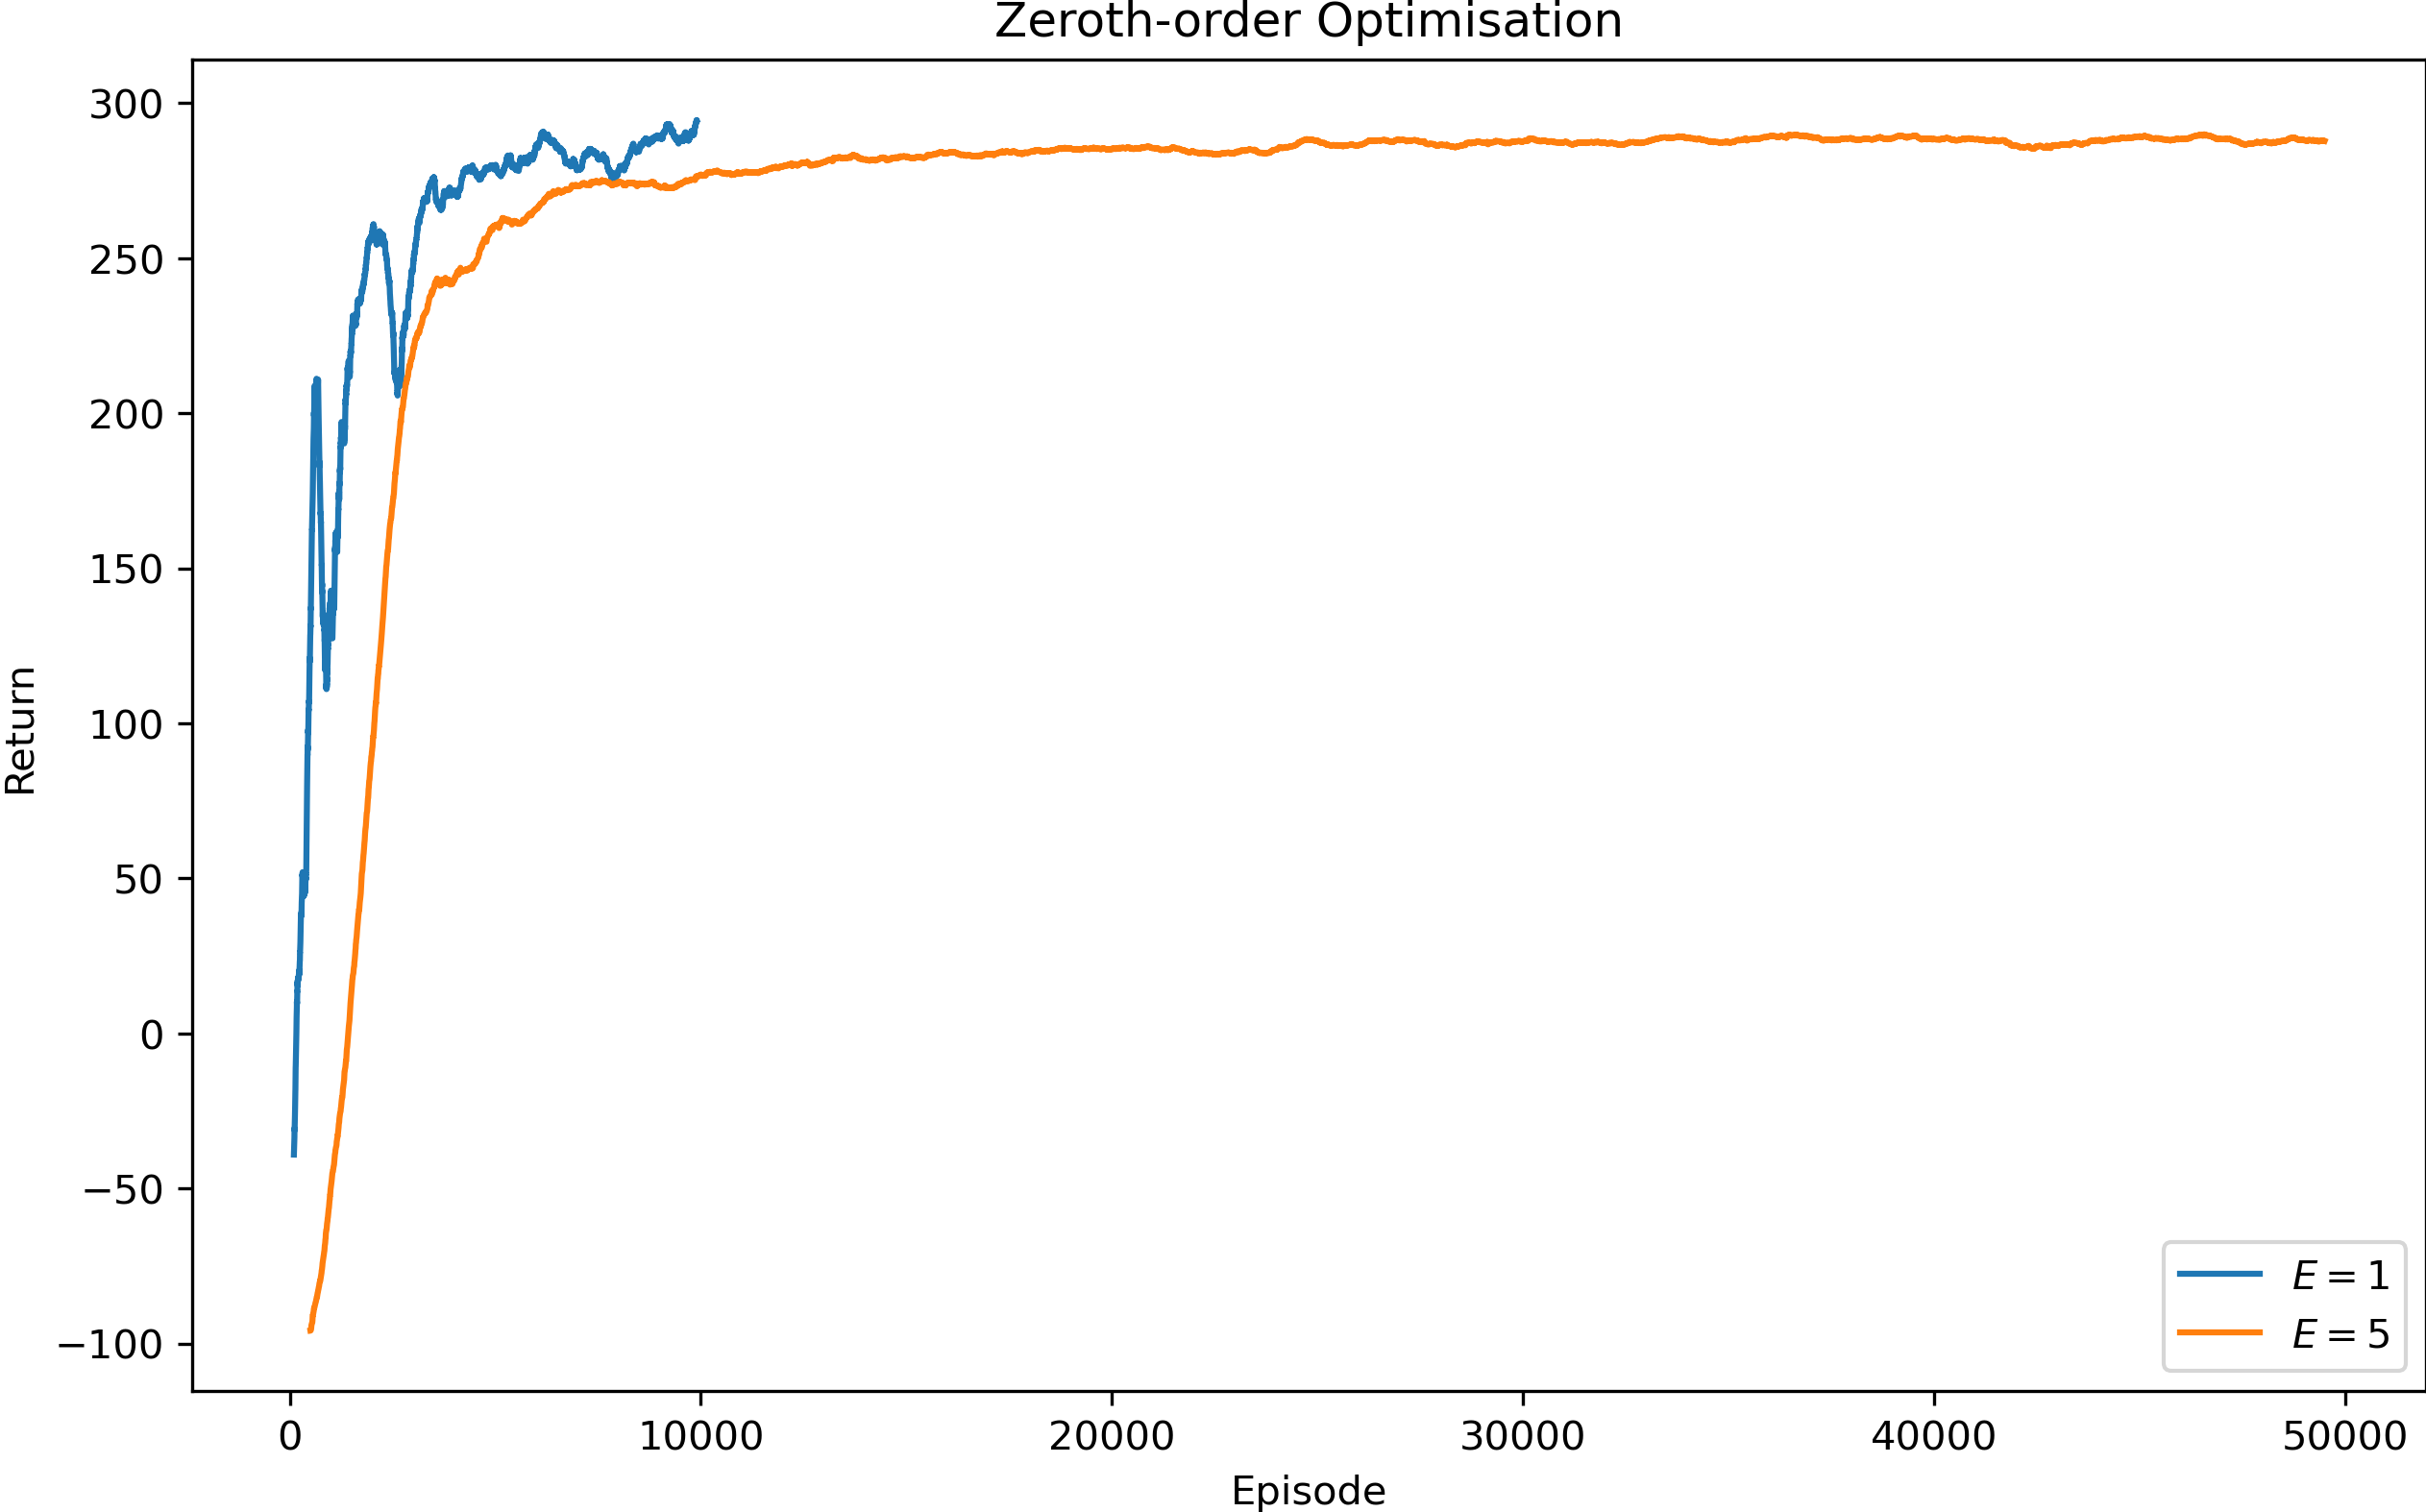
\includegraphics[width=0.9\textwidth]{checkpoints/FINAL/zeroth_order.png}
    \caption{Cumulative reward per evaluation episode for the zeroth-order agents (averaged over 200 iterations)}
    \label{fig:zeroth_order}
\end{figure}

Turning to Figure \ref{fig:population} displaying the results of the population-based agents, we see
the combined influence of the population size $N$ and the number of evaluation episodes $E$ on the performance.
The population-based method can achieve a solving policy in about the 10 times the number of evaluation episodes as the zeroth-order method, but not all agents manage to consistently achieve the same high-quality returns above 275.\\
As far as the influence of the population size $N$ is concerned for $E=1$, we see that the methods
with bigger populations seem to find a successful policy in about the same number of evaluation episodes
as variants with smaller populations
(bigger populations naturally require more evaluations per iteration).
However, it does look like they can learn higher-quality policies due to extra exploration in the same amount of iterations.\\
When we look at the agents that use 5 evaluation episodes, it becomes clear that they learn a successful policy
slightly slower but they are able to improve upon it to obtain higher rewards. Their learning curves are
smoother and increasing the population size does not seem to improve their performance.

\begin{figure}[h]
    \centering
    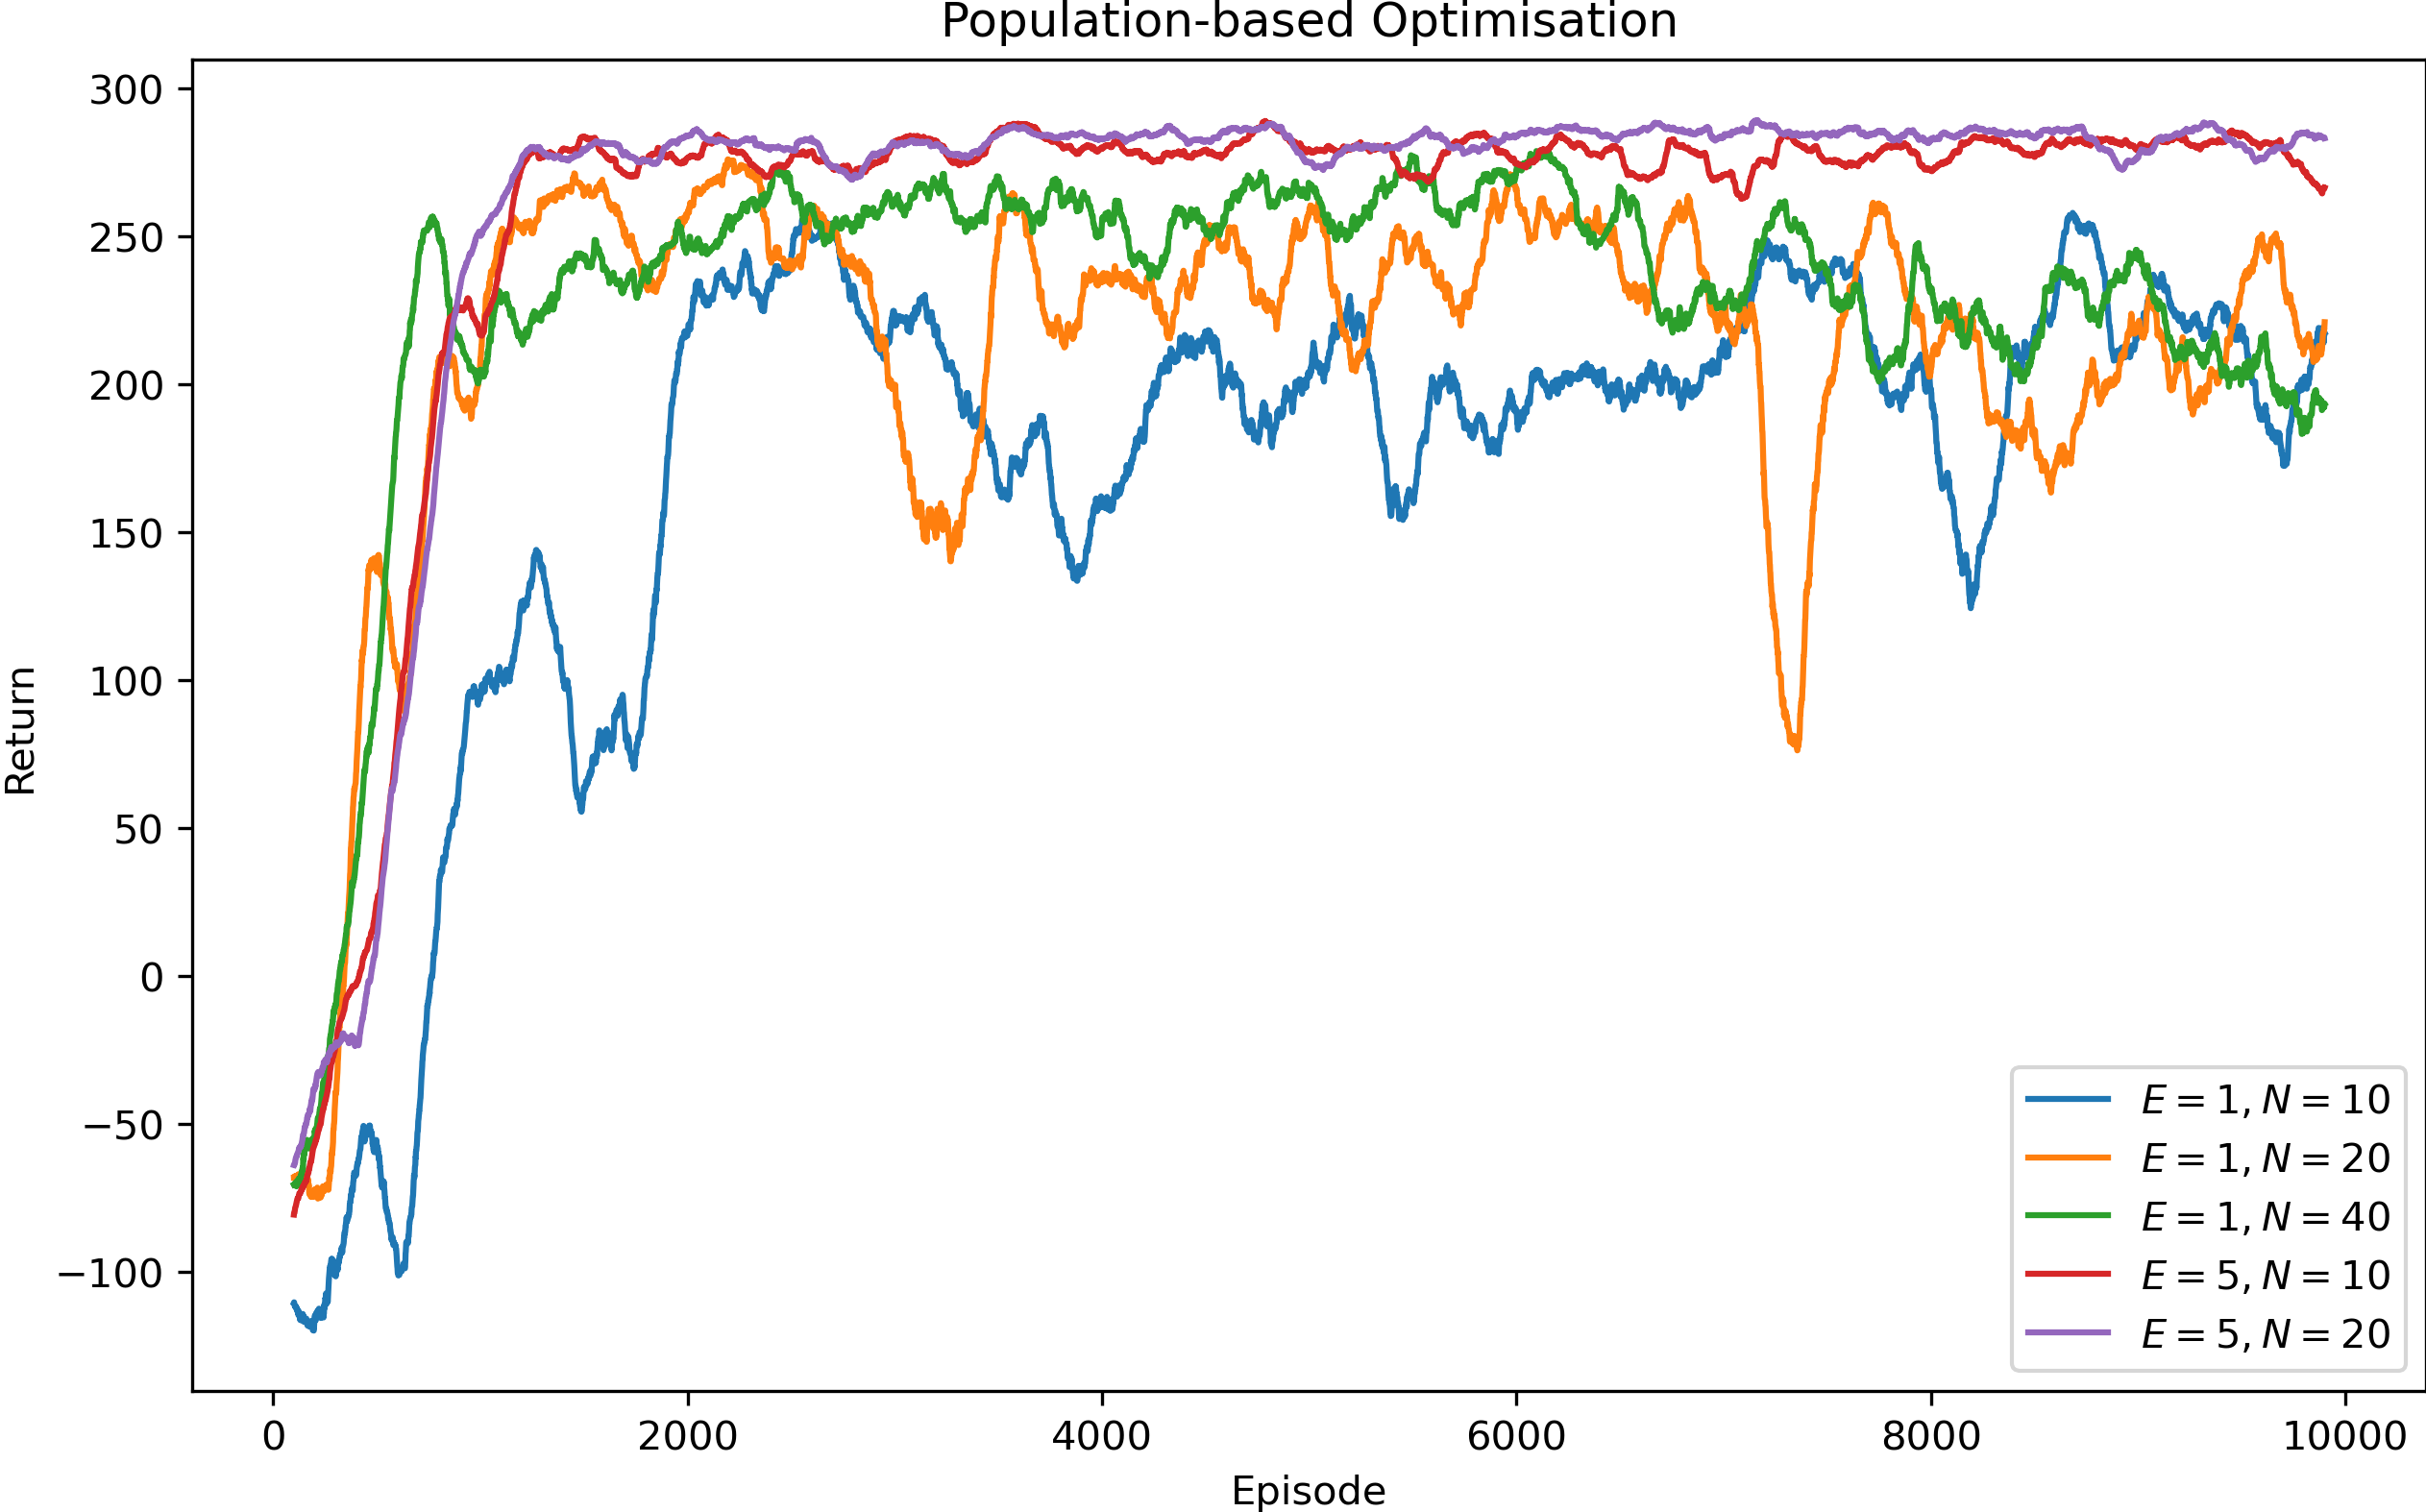
\includegraphics[width=0.9\textwidth]{checkpoints/FINAL/population.png}
    \caption{Cumulative reward per evaluation episode for the population-based agents (averaged over 200 iterations)}
    \label{fig:population}
\end{figure}

\section{Conclusion}

Although gradient-free optimisation methods are not as popular or sofisticated as gradient-based methods in reinfocement learning, they can still make effective agents that are able to learn solving policies in a reasonable amount of time while avoiding the need for a gradient estimator.\\
We have implemented two such methods, the zeroth-order method and the population-based method, and compared their performance in the continuous Lunar Lander environment.
We observed that the zeroth-order method is able to learn a solving policy in about 10 times less evaluation episodes than the population-based method and is less sensitive to the setting of the hyper-parameters.
As one could expect, increasing the number of evaluation episodes per iteration improve the stability of the convergence to an optimal policy at the cost of slowing down the learning process.
For the population-based method, we found that increasing the population size does not necessarily improve the learning speed of the agent but it does allow it to explore the environment more and find higher quality policies. This again comes at the cost of slowing down the learning process.\\
For the zeroth-order method, using only one evaluation episode per iteration seemed to allow the agent to learn faster and does not seem to decrease the quality of the final policy due to environmental noise.\\
On the other hand, in tuning the population-based method, one needs to make a choice between learning
fast with only one evaluation episode per iteration and a achieving a low quality solution or learning slower to obtain a higher quality policy.\\
In conclusion, out of the two methods, the zeroth-order method seems to be the the most sample efficient and the most robust to hyper-parameter tuning.

% bibliography
\bibliographystyle{plain}
\bibliography{report}

\end{document}
